%
% $RCSfile: abstraction_gaps.tex,v $
%
% Copyright (C) 2002-2008. Christian Heller.
%
% Permission is granted to copy, distribute and/or modify this document
% under the terms of the GNU Free Documentation License, Version 1.1 or
% any later version published by the Free Software Foundation; with no
% Invariant Sections, with no Front-Cover Texts and with no Back-Cover
% Texts. A copy of the license is included in the section entitled
% "GNU Free Documentation License".
%
% http://www.cybop.net
% - Cybernetics Oriented Programming -
%
% http://www.resmedicinae.org
% - Information in Medicine -
%
% Version: $Revision: 1.1 $ $Date: 2008-08-19 20:41:05 $ $Author: christian $
% Authors: Christian Heller <christian.heller@tuxtax.de>
%

\section{Abstraction Gaps}
\label{abstraction_gaps_heading}
\index{Abstraction Gaps}
\index{Software Engineering Process}
\index{SEP}
\index{Analysis}
\index{Design}
\index{Implementation}
\index{informal}
\index{Requirements Document}
\index{semi-formal}
\index{Architecture Diagrams}
\index{Unified Modeling Language}
\index{UML}
\index{top-down}
\index{bottom-up}
\index{Yo-Yo}
\index{Source Code}
\index{formal}
\index{Feature Modelling}
\index{Feature Model}
\index{System Family Engineering}
\index{Traceability}
\index{Conceptual Ontology Representation}
\index{Semantic Gaps}
\index{Conceptual Gaps}
\index{Intentionality}
\index{Software Engineering}

Software has to be developed in a creative process (methodology) called
\emph{Software Engineering Process} (SEP). As the previous sections tried to
show, many different forms of such processes exist. Every project, consciously
or not, follows a SEP that sooner-or-later, in one form or the other, goes through
the three common phases \emph{Analysis}, \emph{Design} and \emph{Implementation}
(figure \ref{gaps_figure}). Each phase creates its own (ideally equivalent)
model of what is to be abstracted in software and it is the differences in
exactly these models that often, actually always cause complications.

The analysis mostly results in a \emph{Requirements Document} which investigates
the problem domain and uses expert knowledge to specify the functionality of
the software to be created. This specification is mostly \emph{informal}, that
is an ordered collection of textual descriptions. Sometimes, \emph{semi-formal}
descriptions such as tables or graphics are used additionally.

It is the aim of the design phase to deliver a clear system architecture with
little redundancies and only few interdependencies, which it may specify by
help of \emph{semi-formal} \emph{Diagrams}. Recent years showed an increased
use of the \emph{Unified Modeling Language} (UML), a collection of diagram
specifications for representing static or dynamic aspects of a system.
Normally, a \emph{top-down} approach is chosen for the design of a system.
Hereby, the overall architecture is considered first, before moving into
details. The less common \emph{bottom-up} design would start the other way
round and first try to build small components to construct the whole system
from. A third possible approach, called \emph{Yo-Yo} \cite{buschmann}, would
mix the two above-mentioned kinds.

Finally, implementation of a system is done \emph{formally}, in (one or more)
programming languages. The retrieved \emph{Source Code} represents the
temporally final abstraction, the software that was to be built.

\begin{figure}[ht]
    \begin{center}
        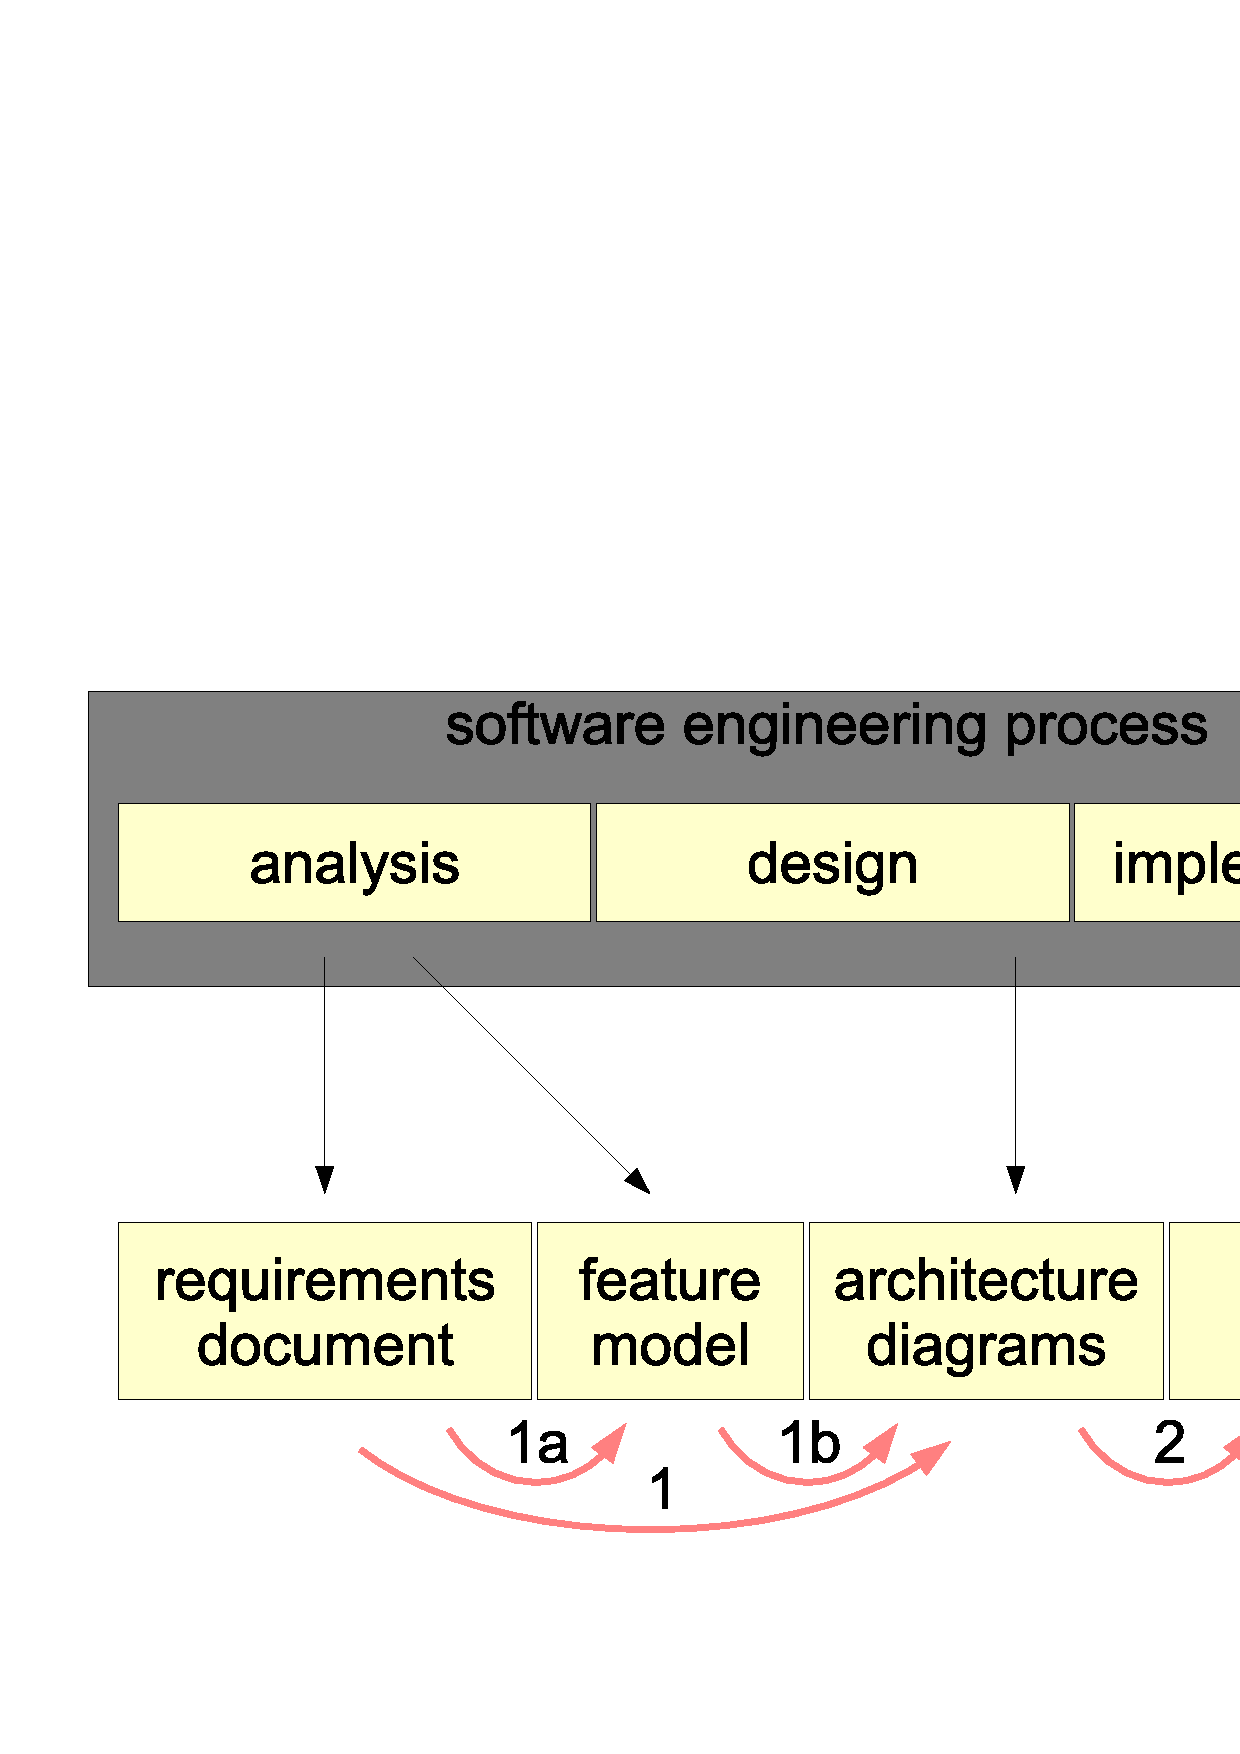
\includegraphics[scale=0.3,angle=-90]{graphic/gaps.pdf}
        \caption{Abstraction Gaps}
        \label{gaps_figure}
    \end{center}
\end{figure}

It is obvious that at least two gaps (figure \ref{gaps_figure}) have to be
crossed when using the described phases:

\begin{enumerate}
    \item Requirements Document -- Architecture Diagrams
    \item Architecture Diagrams -- Source Code
\end{enumerate}

Many efforts try to minimise the first gap by telling their analysis experts
to specify use cases, workflows and static structures using the corresponding
diagrams provided by the \emph{Unified Modeling Language} (UML). Other efforts
like the \emph{Feature Modelling} that became especially popular in the area of
\emph{Product Line-}/ \emph{System Family Engineering} \cite{boellert} introduce
an intermediate step of abstraction. The feature modelling itself is part of the
analysis but can logically be placed between analysis and design. The results it
delivers are called \emph{Feature Models} \cite{streitferdt, pashov}. They
provide hierarchical structures of the design properties of the system to be
built. By applying feature models, the former big abstraction gap is broken down
into two smaller ones (figure \ref{gaps_figure}), that are easier to cross:

\begin{enumerate}
    \item[1a] Requirements Document -- Feature Model
    \item[1b] Feature Model -- Architecture Diagrams
    \item[2] Architecture Diagrams -- Source Code
\end{enumerate}

That way, the \emph{Traceability} between concrete requirements and architecture
components can be improved. Moreover, the \emph{Communication} between
stakeholders in the development process can profit from feature models because
of their closeness to both, analysis and design. Yet has the usage of feature
models one disadvantage, too: another gap in abstraction is created through them.

The same happens in \cite{funkat}, where a special knowledge level called
\emph{Conceptual Ontology Representation}, comparable in its aims to the feature
model, gets introduced as additional abstraction step. The aim of becoming more
independent from implementation code for retrieving a human-readable form of
knowledge, to improve communication between domain experts and engineers may
well be reached, but sooner-or-later, also these models have to be transferred
into program source code, by bridging the classical abstraction gaps mentioned
above.

Bridging or closing these abstraction gaps (sometimes called \emph{Semantic Gaps}
or \emph{Conceptual Gaps} \cite{czarnecki}) is also known as: \textit{achieving
higher intentionality} \cite{czarnecki} and remains an unsolved issue and task
for software engineering. One aim of this work is to try to contribute to a
possible solution, with special focus on \emph{reducing} gap 2, existing
between a designed system architecture and the implemented source code.
